\documentclass[article,A4,12pt]{llncs}

% Conditional compilation.
% NOTE: If you set fullversionfalse, just compile ONCE so that TOC stays unchanged.
\newif\iffullversion
\fullversiontrue
%\fullversionfalse

\usepackage[T1]{fontenc}
\usepackage{amsmath}
\usepackage{amssymb}
\usepackage{color}
\usepackage{amsfonts}
\usepackage{mathrsfs, bm}

\usepackage{graphicx}
\usepackage{tabularx}
\usepackage{subfig}
\usepackage{epsf,times}
\usepackage{color}
\usepackage{wrapfig}
\usepackage{cases}
\usepackage{multicol}
\usepackage[usenames,dvipsnames]{xcolor}

\usepackage{palatino}

\usepackage[T1]{fontenc}
%\newcommand{\tmname}[1]{\textsc{#1}}
%\newcommand{\tmop}[1]{\ensuremath{\operatorname{#1}}}
%\newcommand{\tmsamp}[1]{\textsf{#1}}
%\newcommand{\tmtextsc}[1]{{\scshape{#1}}}
%\newcommand{\tmtextsl}[1]{{\slshape{#1}}}
%\newcommand{\tmtexttt}[1]{{\ttfamily{#1}}}

\leftmargin=0.0cm
\oddsidemargin=0.5cm
\evensidemargin=0.5cm
\topmargin=0cm
\textwidth=16.0cm
%\textheight=21.5cm
\textheight=20.0cm
\pagestyle{plain}
\setlength{\columnsep}{20pt}

\def\m{\mathbf{m}}
\def\H{\mathbf{H}}
\def\E{\mathbf{E}}
\newcommand{\vepsi}{{\varepsilon}}
\def\hnorm#1#2{\vert\,#1\,\vert_{#2}}
\newcommand{\R}{{\mathbb R}}
\newcommand{\Sph}{{\mathbb S}}
\def\x{\mathbf{x}}
\def\hvec{\overline{\mathbf{h}}}
\def\evec{\overline{\mathbf{e}}}

\newcommand{ \etal}{\mbox{\emph{et al. }}}

\newcommand\vect[1]{\mbf{#1}}
\newcommand{\mbf}[1]{\mbox{\boldmath$#1$}} 
\newcommand{\RC}[1]{#1 $\times$ #1 $\times$ #1}
\def\um{$\mu$m}
\def\C{$^{\circ}\mathrm{C}$}

\newcommand{\Rmnum}[1]{\expandafter\@slowromancap\romannumeral #1@}

% DEFINITION OF CUSTOM FONT SIZE
\newcommand{\customfontA}{\fontsize{50}{55}\selectfont}
\newcommand{\customfontB}{\fontsize{14.4}{20}\selectfont}
\newcommand{\customfontC}{\fontsize{30}{35}\selectfont}

\DeclareMathAlphabet{\mathpzc}{OT1}{pzc}{m}{it}

\def\clovek#1{\noindent\bgroup\vbox{\noindent#1}\egroup\vskip1em}





% TO INPUT BACKGROUND IMAGE
%\usepackage{eso-pic}
%\newcommand\BackgroundPic{
%\put(0,0){
%\parbox[b][\paperheight]{\paperwidth}{
%\vfill
%\centering
%\includegraphics[width=\paperwidth,height=\paperheight]{img/karel-frontpage.png}
%%\includegraphics[width=\paperwidth,height=\paperheight]{img/background.jpg}
%\vfill
%}}}

\usepackage{fancyvrb}

\newenvironment{bluecode}{\VerbatimEnvironment \color{blue} \begin{Verbatim}}
{\end{Verbatim}}
\newenvironment{greencode}{\VerbatimEnvironment \color{ForestGreen} \begin{Verbatim}}
{\end{Verbatim}}
\newenvironment{redcode}{\VerbatimEnvironment \color{Red} \begin{Verbatim}}
{\end{Verbatim}}

% For Pygments:
\usepackage{fancyvrb}
\usepackage{color}
\usepackage[utf-8]{inputenc}

\makeatletter
\def\PY@reset{\let\PY@it=\relax \let\PY@bf=\relax%
    \let\PY@ul=\relax \let\PY@tc=\relax%
    \let\PY@bc=\relax \let\PY@ff=\relax}
\def\PY@tok#1{\csname PY@tok@#1\endcsname}
\def\PY@toks#1+{\ifx\relax#1\empty\else%
    \PY@tok{#1}\expandafter\PY@toks\fi}
\def\PY@do#1{\PY@bc{\PY@tc{\PY@ul{%
    \PY@it{\PY@bf{\PY@ff{#1}}}}}}}
\def\PY#1#2{\PY@reset\PY@toks#1+\relax+\PY@do{#2}}

\def\PY@tok@gd{\def\PY@tc##1{\textcolor[rgb]{0.63,0.00,0.00}{##1}}}
\def\PY@tok@gu{\let\PY@bf=\textbf\def\PY@tc##1{\textcolor[rgb]{0.50,0.00,0.50}{##1}}}
\def\PY@tok@gt{\def\PY@tc##1{\textcolor[rgb]{0.00,0.25,0.82}{##1}}}
\def\PY@tok@gs{\let\PY@bf=\textbf}
\def\PY@tok@gr{\def\PY@tc##1{\textcolor[rgb]{1.00,0.00,0.00}{##1}}}
\def\PY@tok@cm{\let\PY@it=\textit\def\PY@tc##1{\textcolor[rgb]{0.25,0.50,0.50}{##1}}}
\def\PY@tok@vg{\def\PY@tc##1{\textcolor[rgb]{0.10,0.09,0.49}{##1}}}
\def\PY@tok@m{\def\PY@tc##1{\textcolor[rgb]{0.40,0.40,0.40}{##1}}}
\def\PY@tok@mh{\def\PY@tc##1{\textcolor[rgb]{0.40,0.40,0.40}{##1}}}
\def\PY@tok@go{\def\PY@tc##1{\textcolor[rgb]{0.50,0.50,0.50}{##1}}}
\def\PY@tok@ge{\let\PY@it=\textit}
\def\PY@tok@vc{\def\PY@tc##1{\textcolor[rgb]{0.10,0.09,0.49}{##1}}}
\def\PY@tok@il{\def\PY@tc##1{\textcolor[rgb]{0.40,0.40,0.40}{##1}}}
\def\PY@tok@cs{\let\PY@it=\textit\def\PY@tc##1{\textcolor[rgb]{0.25,0.50,0.50}{##1}}}
\def\PY@tok@cp{\def\PY@tc##1{\textcolor[rgb]{0.74,0.48,0.00}{##1}}}
\def\PY@tok@gi{\def\PY@tc##1{\textcolor[rgb]{0.00,0.63,0.00}{##1}}}
\def\PY@tok@gh{\let\PY@bf=\textbf\def\PY@tc##1{\textcolor[rgb]{0.00,0.00,0.50}{##1}}}
\def\PY@tok@ni{\let\PY@bf=\textbf\def\PY@tc##1{\textcolor[rgb]{0.60,0.60,0.60}{##1}}}
\def\PY@tok@nl{\def\PY@tc##1{\textcolor[rgb]{0.63,0.63,0.00}{##1}}}
\def\PY@tok@nn{\let\PY@bf=\textbf\def\PY@tc##1{\textcolor[rgb]{0.00,0.00,1.00}{##1}}}
\def\PY@tok@no{\def\PY@tc##1{\textcolor[rgb]{0.53,0.00,0.00}{##1}}}
\def\PY@tok@na{\def\PY@tc##1{\textcolor[rgb]{0.49,0.56,0.16}{##1}}}
\def\PY@tok@nb{\def\PY@tc##1{\textcolor[rgb]{0.00,0.50,0.00}{##1}}}
\def\PY@tok@nc{\let\PY@bf=\textbf\def\PY@tc##1{\textcolor[rgb]{0.00,0.00,1.00}{##1}}}
\def\PY@tok@nd{\def\PY@tc##1{\textcolor[rgb]{0.67,0.13,1.00}{##1}}}
\def\PY@tok@ne{\let\PY@bf=\textbf\def\PY@tc##1{\textcolor[rgb]{0.82,0.25,0.23}{##1}}}
\def\PY@tok@nf{\def\PY@tc##1{\textcolor[rgb]{0.00,0.00,1.00}{##1}}}
\def\PY@tok@si{\let\PY@bf=\textbf\def\PY@tc##1{\textcolor[rgb]{0.73,0.40,0.53}{##1}}}
\def\PY@tok@s2{\def\PY@tc##1{\textcolor[rgb]{0.73,0.13,0.13}{##1}}}
\def\PY@tok@vi{\def\PY@tc##1{\textcolor[rgb]{0.10,0.09,0.49}{##1}}}
\def\PY@tok@nt{\let\PY@bf=\textbf\def\PY@tc##1{\textcolor[rgb]{0.00,0.50,0.00}{##1}}}
\def\PY@tok@nv{\def\PY@tc##1{\textcolor[rgb]{0.10,0.09,0.49}{##1}}}
\def\PY@tok@s1{\def\PY@tc##1{\textcolor[rgb]{0.73,0.13,0.13}{##1}}}
\def\PY@tok@sh{\def\PY@tc##1{\textcolor[rgb]{0.73,0.13,0.13}{##1}}}
\def\PY@tok@sc{\def\PY@tc##1{\textcolor[rgb]{0.73,0.13,0.13}{##1}}}
\def\PY@tok@sx{\def\PY@tc##1{\textcolor[rgb]{0.00,0.50,0.00}{##1}}}
\def\PY@tok@bp{\def\PY@tc##1{\textcolor[rgb]{0.00,0.50,0.00}{##1}}}
\def\PY@tok@c1{\let\PY@it=\textit\def\PY@tc##1{\textcolor[rgb]{0.25,0.50,0.50}{##1}}}
\def\PY@tok@kc{\let\PY@bf=\textbf\def\PY@tc##1{\textcolor[rgb]{0.00,0.50,0.00}{##1}}}
\def\PY@tok@c{\let\PY@it=\textit\def\PY@tc##1{\textcolor[rgb]{0.25,0.50,0.50}{##1}}}
\def\PY@tok@mf{\def\PY@tc##1{\textcolor[rgb]{0.40,0.40,0.40}{##1}}}
\def\PY@tok@err{\def\PY@bc##1{\fcolorbox[rgb]{1.00,0.00,0.00}{1,1,1}{##1}}}
\def\PY@tok@kd{\let\PY@bf=\textbf\def\PY@tc##1{\textcolor[rgb]{0.00,0.50,0.00}{##1}}}
\def\PY@tok@ss{\def\PY@tc##1{\textcolor[rgb]{0.10,0.09,0.49}{##1}}}
\def\PY@tok@sr{\def\PY@tc##1{\textcolor[rgb]{0.73,0.40,0.53}{##1}}}
\def\PY@tok@mo{\def\PY@tc##1{\textcolor[rgb]{0.40,0.40,0.40}{##1}}}
\def\PY@tok@kn{\let\PY@bf=\textbf\def\PY@tc##1{\textcolor[rgb]{0.00,0.50,0.00}{##1}}}
\def\PY@tok@mi{\def\PY@tc##1{\textcolor[rgb]{0.40,0.40,0.40}{##1}}}
\def\PY@tok@gp{\let\PY@bf=\textbf\def\PY@tc##1{\textcolor[rgb]{0.00,0.00,0.50}{##1}}}
\def\PY@tok@o{\def\PY@tc##1{\textcolor[rgb]{0.40,0.40,0.40}{##1}}}
\def\PY@tok@kr{\let\PY@bf=\textbf\def\PY@tc##1{\textcolor[rgb]{0.00,0.50,0.00}{##1}}}
\def\PY@tok@s{\def\PY@tc##1{\textcolor[rgb]{0.73,0.13,0.13}{##1}}}
\def\PY@tok@kp{\def\PY@tc##1{\textcolor[rgb]{0.00,0.50,0.00}{##1}}}
\def\PY@tok@w{\def\PY@tc##1{\textcolor[rgb]{0.73,0.73,0.73}{##1}}}
\def\PY@tok@kt{\def\PY@tc##1{\textcolor[rgb]{0.69,0.00,0.25}{##1}}}
\def\PY@tok@ow{\let\PY@bf=\textbf\def\PY@tc##1{\textcolor[rgb]{0.67,0.13,1.00}{##1}}}
\def\PY@tok@sb{\def\PY@tc##1{\textcolor[rgb]{0.73,0.13,0.13}{##1}}}
\def\PY@tok@k{\let\PY@bf=\textbf\def\PY@tc##1{\textcolor[rgb]{0.00,0.50,0.00}{##1}}}
\def\PY@tok@se{\let\PY@bf=\textbf\def\PY@tc##1{\textcolor[rgb]{0.73,0.40,0.13}{##1}}}
\def\PY@tok@sd{\let\PY@it=\textit\def\PY@tc##1{\textcolor[rgb]{0.73,0.13,0.13}{##1}}}

\def\PYZbs{\char`\\}
\def\PYZus{\char`\_}
\def\PYZob{\char`\{}
\def\PYZcb{\char`\}}
\def\PYZca{\char`\^}
\def\PYZsh{\char`\#}
\def\PYZpc{\char`\%}
\def\PYZdl{\char`\$}
\def\PYZti{\char`\~}
% for compatibility with earlier versions
\def\PYZat{@}
\def\PYZlb{[}
\def\PYZrb{]}
\makeatother
% End of Pygments inputs.

% Define color boxes:
\definecolor{MyGreen}{rgb}{0.9, 1, 0.9}
\makeatletter\newenvironment{gbox}{%
   \begin{lrbox}{\@tempboxa}\begin{minipage}{0.985\columnwidth}}{\end{minipage}\end{lrbox}%
   \noindent
   \colorbox{MyGreen}{\usebox{\@tempboxa}}
}\makeatother

%\definecolor{MyYellow}{rgb}{0.98, 0.98, 0.824}
\definecolor{MyYellow}{rgb}{1, 0.99, 0.8}
\makeatletter\newenvironment{ybox}{%
   \begin{lrbox}{\@tempboxa}\begin{minipage}{0.985\columnwidth}}
   {\end{minipage}\end{lrbox}%
   \noindent
   \colorbox{MyYellow}{\usebox{\@tempboxa}}
}\makeatother

\definecolor{MyBlue}{rgb}{0.88, 0.95, 1}
\makeatletter\newenvironment{bbox}{%
   \begin{lrbox}{\@tempboxa}\begin{minipage}{0.985\columnwidth}}
   {\end{minipage}\end{lrbox}%
   \noindent
   \colorbox{MyBlue}{\usebox{\@tempboxa}}
}\makeatother

\definecolor{MyBlue}{rgb}{0.88, 0.95, 1}
\makeatletter\newenvironment{bboxshort}{%
   \begin{lrbox}{\@tempboxa}\begin{minipage}{0.95\columnwidth}}
   {\end{minipage}\end{lrbox}%
   \noindent
   \colorbox{MyBlue}{\usebox{\@tempboxa}}
}\makeatother


\usepackage{wallpaper}


\begin{document}


%%%%%%%%%%%%%%%%%%%%%%%%%%%%%%%%%%%%%%%%%%%%%%%%%%%%%%%%%%%%%%%%%%%%%%%%%
\pagestyle{empty}

\ThisULCornerWallPaper{1.02}{img/karel-cover.png}






%%%%%%%%%%%%%%%%%%%%%%%%%%%%%%%%%%%%%%%%%%%%%%%%%%%%%%%%%%%%%%%%%%%%%%%%%
\newpage
\vbox{}
\newpage
\vbox{}
\vfill

\centerline{Revision Feb-16-2013}

%%%%%%%%%%%%%%%%%%%%%%%%%%%%%%%%%%%%%%%%%%%%%%%%%%%%%%%%%%%%%%%%%%%%%%%%%
\newpage

\noindent
{\bf About this Textbook}\\[2mm]
This free textbook is provided as a courtesy to NCLab users. It will help you develop 
{\em algorithmic thinking} which is the most challenging skill to acquire when learning 
computer programming. Once you are able to "think like a computer", learning 
any computer language is almost effortless. Karel is a famous educational language created and still used at 
the Stanford University. After taking this course, you will be able to transition swiftly 
to Python and other modern programming languages. \\[2mm]

\noindent
{\bf Become a Co-Author}\\[2mm]
We do not plan to publish the textbook with a commercial publisher since this 
would make it unnecessarily expensive for kids and students who are the main 
target audience. Feel free to contribute to the textbook with any material or 
suggestions. There is never enough illustrations and exercises, and there always 
are bugs to report. Translating the textbook into other languages would benefit
thousands of kids worldwide. Instructions for contributors can be found 
below.\\[2mm]

\noindent
{\bf How to Contribute (for \LaTeX \ and Git users)}\\[2mm]
\noindent
The textbook is written in \LaTeX, a high-quality typesetting system that 
you can learn and use in NCLab. In the future it will be possible to contribute to 
the textbook directly in NCLab, but at this time, the sources are stored 
in a public Git repository {\tt nclab-textbook-karel} at Github (http://github.com). \\[2mm]

\noindent
{\bf How to Contribute (for all others)}\\[2mm]
\noindent
We will gladly accept new interesting exercises for Karel and/or Python, as well as
new images of good quality that will make the textbook more interesting and fun. You
can send those at any time via email to {\tt pavel@femhub.com}.\\[2mm]

\noindent
{\bf List of Contributors}
\begin{itemize}
\item Pavel Solin, University of Nevada, Reno (primary author). 
\item Martin Novak, Czech Technical University, Prague, Czech Republic.
\item Salih Dede, Coral Academy of Science High School, Reno, NV.
\item Nazhmiddin Shapoatov, Sonoran Science Academy, Phoenix, AZ.
\item Veronica McVey, Winnemucca Junior High School, NV.
\item Jozsef Hollosi, Westfield, NJ.
\item Ed Keppelmann, Reno, NV.
\end{itemize}
\vspace{2mm}
\noindent
{\bf Graphics Design:} TR-Design {\tt http://tr-design.cz}

%\noindent
%{\bf For Instructors}\\[4mm]
%Review Book and Exercise Book containing 
%review questions with answers and programming exercises with
%solutions, are part of the NCLab-powered course 
%{\em Intro to Programming with Karel the Robot and Python} that is 
%available at \\[4mm]
%
%{\color{blue}
%\centerline{\tt http://introtoprogramming.net}
%}
%\vspace{5mm}
%
%\noindent
%for a small subscription fee. The fee is used to cover cloud computing resources, 
%development, maintenance, and user support. 
%
%The course is completely web-browser based, no installation of anything at your school 
%or home is needed. You and your students can access the course from anywhere and at any 
%time. Instructor's workflow includes downloading assignments and review
%question worksheets from the database, sending them to the students 
%via one mouse click, and collecting them back, automatically graded. 
%The course is scheduled to open in January 2013. In the meantime, enjoy 
%Karel and Python, and let us know with any questions at {\tt support@nclab.com}!


\newpage
%{\ }
\setcounter{tocdepth}{2}
\tableofcontents
%\pagestyle{plain}

\newpage

\pagestyle{plain}
\setcounter{page}{1}

%%%%%%%%%%%%%%%%%%%%%%%%%%%%%%%%%%%%%%%%%%%%%%%%%%%%%%%%%%%%%%%%%%%%%%%%%
\pagestyle{plain}
\setcounter{page}{1}
\section*{Foreword}

This course provides an efficient introduction to modern algorithmic design and computer programming
using the legendary educational programming language {\em Karel the Robot}. The language was 
first introduced by Richard E. Pattis at Stanford University in his famous book {\em Karel the Robot: 
A Gentle Introduction to the Art of Programming}. 


With Karel, learning feels more like playing. 
You will not be exposed to discouraging 
technical complications of conventional programming languages or mathematics, 
and in no time you will get used to "thinking like a computer". This essential skill, otherwise
known as {\em algorithmic thinking}, is much more important for computer programming than knowledge 
of any particular programming language. 

We have seen many students struggle with computer programming and we know that there is 
absolutely no need for that. Often the only problem is the widely adopted mistake
of instructors who use a powerful mainstream programming language such as Java, C or even C++ 
for a first programming course. This, however, is similar to teaching someone how to ride 
a motorcycle without teaching him or her how to ride a bicycle first. While there is nothing 
wrong with motorcycles, a beginner needs to learn to keep the balance first, and for that the
motorcycle simply may not be the best tool.

\begin{figure}[!ht]
\begin{center}
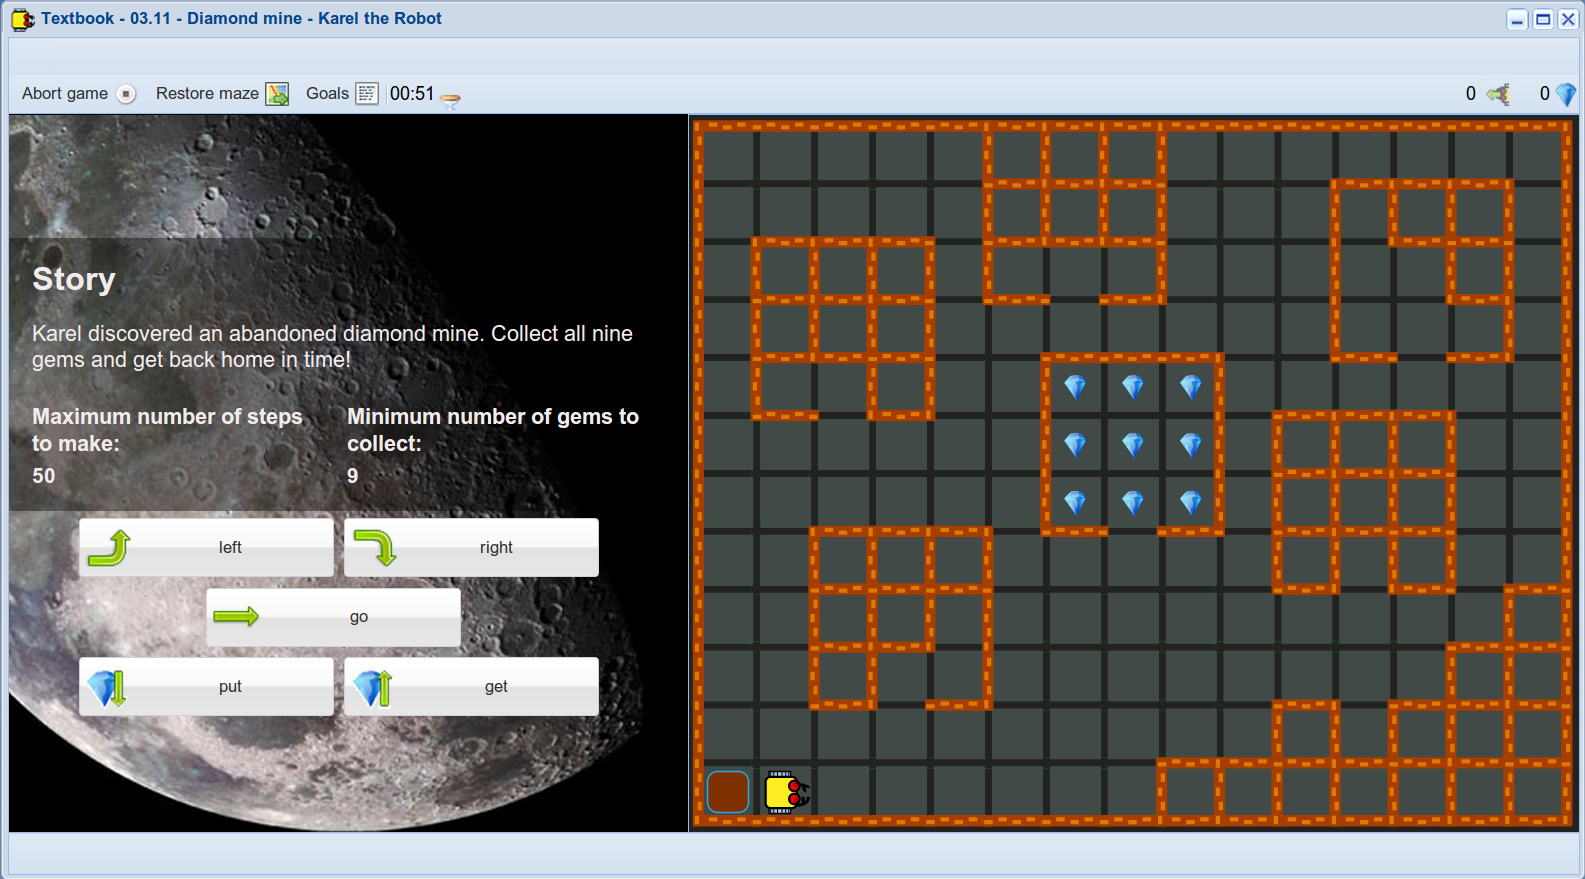
\includegraphics[width=0.75\textwidth]{img/fore-1.png}
\end{center}
\vspace{-2mm}
\caption{Sample game {\em Diamond Mine} in Manual mode.}
\label{fig:f1}
\vspace{-4mm}
\end{figure}
\noindent
Learning to ride a bicycle before riding a motorbike is exactly what Karel the Robot is 
about. The robot only knows a handful of simple commands and has a few sensors to navigate 
through the maze. There is no mathematics or confusing technicalities of conventional 
programming languages to worry about. 

The course starts out in Manual mode (Level 0) where the robot can be guided via 
clicking on five buttons {\em Go} (make one step forward), {\em Left} (turn left), {\em Right} 
(turn right), {\em Put} (put a gem on the groud) and {\em Get} (pick up a gem from the ground). 
In the next level which is called {\em Bridge to Programming} students keep solving 
problems by typing the commands {\tt go}, {\tt left}, {\tt right}, {\tt put} and {\tt get} 
instead of clicking on buttons. 

The need for higher functionality such as loops, conditions, and custom commands arises 
naturally as game goals become more complicated. 
Students learn quickly that it is advantageous to break complex tasks into smaller 
ones, which is one of the most important principle of computer 
programming. The textbook is written by programming experts, and in addition to 
advanced programming skills the students gain an overview of good and bad 
programming habits.

\begin{figure}[!ht]
\begin{center}
\includegraphics[width=0.75\textwidth]{img/fore-2.png}
\end{center}
\vspace{-2mm}
\caption{Sample game {\em Speleologist} in Programming mode.}
\label{fig:f2}
\vspace{-4mm}
\end{figure}
\noindent
The syntax of Karel the Robot is very close to Python, a modern high-level dynamic 
programming language that is widely used in science, engineering, business and other
areas today. In fact Python feels like Karel's
older brother -- the transition from Karel to Python is as seamless as the transition from 
one Karel's Level to another. 

\part{Meet Karel}

\input textbook.tex

\part{Programming Exercises}
\setcounter{section}{0}

\input exercises.tex

\part{Review Questions}
\setcounter{section}{0}

\input review-questions.tex

\end{document}
